\documentclass{article}
\usepackage[UTF8]{ctex}
\usepackage[T1]{fontenc}
\usepackage[utf8]{inputenc}
\usepackage{float}
\usepackage{placeins}
\usepackage{latexsym}
\usepackage{amsmath}
\usepackage{amsthm}
\usepackage{amssymb}
\usepackage{tikz}
\usepackage{subfigure}
\usepackage{hyperref}

\usetikzlibrary{arrows}

\tikzset{
  treenode/.style = {align=center, inner sep=0pt, text centered, font=\ttfamily},
  BlackNode/.style = {treenode, circle, white, font = \ttfamily\bfseries, draw = black, fill = black, text width = 1.5em},
  RedNode/.style = {treenode, circle, white, font = \ttfamily\bfseries, draw = red, fill = red, text width=1.5em},
  Nil/.style = {treenode, circle, draw = black, minimum width=0.5em, minimum height=0.5em}
}
\allowdisplaybreaks[2]

\hypersetup{
    colorlinks=true,
    linkcolor = black,
    urlcolor=blue!30!green,
}

\title{Homework 5}
\author{PB17000297 罗晏宸}
\date{October 19 2019}



\begin{document}

\maketitle

\section{Exercise 11.3-4}
考虑一个大小为$m = 1000$的散列表和一个对应的散列函数$h(k) = \lfloor m(kA\ \text{mod}\ 1) \rfloor$,其中$A = (\sqrt{5} − 1)/2$,试计算关键字61, 62, 63, 64和65被映射到的位置。
\paragraph{解}
由散列函数,代入关键字计算如下:
\begin{align*}
    h(61)
        &= \lfloor m(kA\ \text{mod}\ 1) \rfloor \\
        &= \left \lfloor 1000 \times \left(61 \times \frac{\sqrt{5}-1}{2} \ \text{mod}\ 1 \right) \right \rfloor \\
        &= \left \lfloor 1000 \times \left( 61 \times \frac{\sqrt{5}-1}{2} - 37 \right) \right \rfloor \\
        &= \left \lfloor 30500\sqrt{5} - 67500 \right \rfloor \\
        &= 700 \\
    \\
    h(62)
        &= \left \lfloor 1000 \times \left(62 \times \frac{\sqrt{5}-1}{2} \ \text{mod}\ 1 \right) \right \rfloor \\
        &= \left \lfloor 31000\sqrt{5} - 69000 \right \rfloor \\
        &= 318 \\
    \\
    h(63)
        &= \left \lfloor 1000 \times \left(63 \times \frac{\sqrt{5}-1}{2} \ \text{mod}\ 1 \right) \right \rfloor \\
        &= \left \lfloor 31500\sqrt{5} - 69500 \right \rfloor \\
        &= 936 \\
        \\
    h(64)
        &= \left \lfloor 1000 \times \left(64 \times \frac{\sqrt{5}-1}{2} \ \text{mod}\ 1 \right) \right \rfloor \\
        &= \left \lfloor 32000\sqrt{5} - 71000 \right \rfloor \\
        &= 554 \\
        \\
    h(65)
        &= \left \lfloor 1000 \times \left(65 \times \frac{\sqrt{5}-1}{2} \ \text{mod}\ 1 \right) \right \rfloor \\
        &= \left \lfloor 32500\sqrt{5} - 72500 \right \rfloor \\
        &= 172 \\
\end{align*}
因此,关键字61, 62, 63, 64和65分别被映射到表中地址为700, 318, 936, 554, 172的位置

\section{Exercise 11.4-1}
考虑用开放寻址法将关键字10, 22, 31, 4, 15, 28, 17, 88, 59插入到一长度为$m = 11$的散列表中,辅助散列函数为$(k) + 0 = k$。试说明分别用线性探查、二次探查($c_1 = 1,\,c_2 = 3$)和双重散列($h_1(k) = k,\,
h_2(k) = 1 + (k\ \text{mod}\ (m − 1))$)将这些关键字插入散列表的过程。

\paragraph{解}
使用三种方式插入关键字的过程与结果如下
\subparagraph{线性探查}
\begin{align*}
    &h(10) &= (10 + 0) \ \text{mod}\  11 &= 10 \\
    \\
    &h(22) &= (22 + 0) \ \text{mod}\  11 &= 0 \\
    \\
    &h(31) &= (31 + 0) \ \text{mod}\  11 &= 9 \\
    \\
    &h(4) &= (4 + 0) \ \text{mod}\  11 &= 4 \\
    \\
    && (15 + 0) \ \text{mod}\  11 &= \mathbf{4} \\
    &h(15) &= (15 + 1) \ \text{mod}\  11 &= 5 \\
    \\
    &h(28) &= (28 + 0) \ \text{mod}\  11 &= 6 \\
    \\
    &&(17 + 0) \ \text{mod}\  11 &= \mathbf{6} \\
    &h(17) &= (17 + 1) \ \text{mod}\  11 &= 7 \\
    \\
    &&(88 + 0) \ \text{mod}\  11 &= \mathbf{0} \\
    &h(88) &= (88 + 1) \ \text{mod}\  11 &= 1 \\
    \\
    &&(59 + 0) \ \text{mod}\  11 &= \mathbf{4} \\
    &&(59 + 1) \ \text{mod}\  11 &= \mathbf{5} \\
    &&(59 + 2) \ \text{mod}\  11 &= \mathbf{6} \\
    &&(59 + 3) \ \text{mod}\  11 &= \mathbf{7} \\
    &h(59) &= (59 + 4) \ \text{mod}\  11 &= 8
\end{align*}
最终散列表如表所示
\begin{table}[H]
    \centering
    \begin{tabular}{|c|c|c|c|c|c|c|c|c|c|c|c|}
    \hline
    地址 & 0 & 1 & 2 & 3 & 4 & 5 & 6 & 7 & 8 & 9 & 10 \\ \hline
    关键字 & 22 & 88 &  &  & 4 & 15 & 28 & 17 & 59 & 31 & 10 \\ \hline
    \end{tabular}
    \caption{使用线性探查将关键字插入散列表}
\end{table}

\subparagraph{二次探查}
\begin{align*}
    &h(10) &= (10 + 1 \times 0 + 3 \times 0^2 ) \ \text{mod}\  11 &= 10 \\
    \\
    &h(22) &= (22 + 1 \times 0 + 3 \times 0^2 ) \ \text{mod}\  11 &= 0 \\
    \\
    &h(31) &= (31 + 1 \times 0 + 3 \times 0^2 ) \ \text{mod}\  11 &= 9 \\
    \\
    &h(4) &= (4 + 1 \times 0 + 3 \times 0^2 ) \ \text{mod}\  11 &= 4 \\
    \\
    && (15 + 1 \times 0 + 3 \times 0^2 ) \ \text{mod}\  11 &= \mathbf{4} \\
    &h(15) &= (15 + 1 \times 1 + 3 \times 1^2 ) \ \text{mod}\  11 &= 8 \\
    \\
    &h(28) &= (28 + 1 \times 0 + 3 \times 0^2 ) \ \text{mod}\  11 &= 6 \\
    \\
    &&(17 + 1 \times 0 + 3 \times 0^2 ) \ \text{mod}\  11 &= \mathbf{6} \\
    &&= (17 + 1 \times 1 + 3 \times 1^2 ) \ \text{mod}\  11 &= \mathbf{7} \\
    &&= (17 + 1 \times 2 + 3 \times 2^2 ) \ \text{mod}\  11 &= \mathbf{8} \\
    &h(17) &= (17 + 1 \times 3 + 3 \times 3^2 ) \ \text{mod}\  11 &= 3 \\
    \\
    &&(88 + 1 \times 0 + 3 \times 0^2 ) \ \text{mod}\  11 &= \mathbf{0} \\
    &&= (88 + 1 \times 1 + 3 \times 1^2 ) \ \text{mod}\  11 &= \mathbf{4} \\
    &&= (88 + 1 \times 2 + 3 \times 2^2 ) \ \text{mod}\  11 &= \mathbf{3} \\
    &&= (88 + 1 \times 3 + 3 \times 3^2 ) \ \text{mod}\  11 &= \mathbf{8} \\
    &&= (88 + 1 \times 4 + 3 \times 4^2 ) \ \text{mod}\  11 &= \mathbf{8} \\
    &&= (88 + 1 \times 5 + 3 \times 5^2 ) \ \text{mod}\  11 &= \mathbf{3} \\
    &&= (88 + 1 \times 6 + 3 \times 6^2 ) \ \text{mod}\  11 &= \mathbf{4} \\
    &&= (88 + 1 \times 7 + 3 \times 7^2 ) \ \text{mod}\  11 &= \mathbf{0} \\
    &h(88) &= (88 + 1 \times 8 + 3 \times 8^2 ) \ \text{mod}\  11 &= 2 \\
    \\
    &&(59 + 1 \times 0 + 3 \times 0^2 ) \ \text{mod}\  11 &= \mathbf{4} \\
    &&= (59 + 1 \times 1 + 3 \times 1^2 ) \ \text{mod}\  11 &= \mathbf{8} \\
    &h(59) &= (59 + 1 \times 2 + 3 \times 2^2 ) \ \text{mod}\  11 &= 7
\end{align*}

最终散列表如表所示
\begin{table}[H]
    \centering
    \begin{tabular}{|c|c|c|c|c|c|c|c|c|c|c|c|}
    \hline
    地址 & 0 & 1 & 2 & 3 & 4 & 5 & 6 & 7 & 8 & 9 & 10 \\ \hline
    关键字 & 22 &  & 88 & 17 & 4 &  & 28 & 59 & 15 & 31 & 10 \\ \hline
    \end{tabular}
    \caption{使用二次探查将关键字插入散列表}
\end{table}

\subparagraph{双重散列}
\begin{align*}
    &h(10) &= \big[10 + 0 \times \big(1 + (10\ \text{mod}\ 10)\big)\big] \ \text{mod}\  11 &= 10 \\
    \\
    &h(22) &= \big[22 + 0 \times \big(1 + (22\ \text{mod}\ 10)\big)\big] \ \text{mod}\  11 &= 0 \\
    \\
    &h(31) &= \big[31 + 0 \times \big(1 + (31\ \text{mod}\ 10)\big)\big] \ \text{mod}\  11 &= 9 \\
    \\
    &h(4) &= \big[4 + 0 \times \big(1 + (4\ \text{mod}\ 10)\big)\big] \ \text{mod}\  11 &= 4 \\
    \\
    &&\big[15 + 0 \times \big(1 + (15\ \text{mod}\ 10)\big)\big] \ \text{mod}\  11 &= \mathbf{4} \\
    &&\big[15 + 1 \times \big(1 + (15\ \text{mod}\ 10)\big)\big] \ \text{mod}\  11 &= \mathbf{10} \\
    &h(15) &= \big[15 + 2 \times \big(1 + (15\ \text{mod}\ 10)\big)\big] \ \text{mod}\  11 &= 5 \\
    \\
    &h(28) &= \big[28 + 0 \times \big(1 + (28\ \text{mod}\ 10)\big)\big] \ \text{mod}\  11 &= 6 \\
    \\
    &&\big[17 + 0 \times \big(1 + (17\ \text{mod}\ 10)\big)\big] \ \text{mod}\  11 &= \mathbf{6} \\
    &h(17) &= \big[17 + 1 \times \big(1 + (17\ \text{mod}\ 10)\big)\big] \ \text{mod}\  11 &= 3 \\
    \\
    &&\big[88 + 0 \times \big(1 + (88\ \text{mod}\ 10)\big)\big] \ \text{mod}\  11 &= \mathbf{0} \\
    &&\big[88 + 1 \times \big(1 + (88\ \text{mod}\ 10)\big)\big] \ \text{mod}\  11 &= \mathbf{9} \\
    &h(88) &= \big[88 + 2 \times \big(1 + (88\ \text{mod}\ 10)\big)\big] \ \text{mod}\  11 &= 7 \\
    \\
    &&\big[59 + 0 \times \big(1 + (59\ \text{mod}\ 10)\big)\big] \ \text{mod}\  11 &= \mathbf{4} \\
    &&\big[59 + 1 \times \big(1 + (59\ \text{mod}\ 10)\big)\big] \ \text{mod}\  11 &= \mathbf{3} \\
    &h(59) &= \big[59 + 2 \times \big(1 + (59\ \text{mod}\ 10)\big)\big] \ \text{mod}\  11 &= 2
\end{align*}

最终散列表如表所示
\begin{table}[H]
    \centering
    \begin{tabular}{|c|c|c|c|c|c|c|c|c|c|c|c|}
    \hline
    地址 & 0 & 1 & 2 & 3 & 4 & 5 & 6 & 7 & 8 & 9 & 10 \\ \hline
    关键字 & 22 &  & 59 & 17 & 4 & 15 & 28 & 88 &  & 31 & 10 \\ \hline
    \end{tabular}
    \caption{使用双重散列将关键字插入散列表}
\end{table}

\section{Exercise 12.1-5}
因为在基于比较的排序模型中,完成$n$个元素的排序,其最坏情况下需要$\Omega(n \lg{n})$时间。试证明:任何基于比较的算法从$n$个元素的任意序列中构造一棵二叉搜索树,其最坏情况下需要$\Omega(n \lg{n})$的时间。

\paragraph{证明}
事实上,我们可以通过先进行一次基于比较的排序,再基于此有序序列构造一个除了唯一的叶子结点外,所有结点有且只有左孩子的二叉搜索树,这样得到的算法在最坏情况下需要$\Omega(n \lg{n})$时间,因此任何基于比较的从$n$个元素的任意序列中构造一棵二叉搜索树的算法,在其最坏情况下需要的时间都不会超过$\Omega(n \lg{n})$
\par
假设有这样一个基于比较的算法可以从$n$个元素的任意序列中构造一棵二叉搜索树,其最坏情况下需要的时间小于$\Omega(n \lg{n})$。已知中序遍历一个二叉搜索树需要的时间为$\Theta(n)$,那么我们可以通过先利用此算法构造二叉搜索树再中序遍历之的方式得到一个在最坏情况下需要的时间小于$\Omega(n \lg{n})$的排序算法,这和已知矛盾,因此假设不成立,即不存在这样的算法可以从$n$个元素的任意序列中构造一棵二叉搜索树,其最坏情况下需要的时间小于$\Omega(n \lg{n})$。
\par
综上,任何基于比较的算法从$n$个元素的任意序列中构造一棵二叉搜索树,其最坏情况下需要$\Omega(n \lg{n})$的时间,证毕。

\section{Exercise 13.4-3}
\subsection*{(a)}
将关键字41, 38, 31, 12, 19, 8连续地插入一棵初始为空的红黑树之后,试画出该结果树。
\subsection*{(b)}
对于(a)中得到的红黑树,依次删除8, 12, 19,试画出每次删除操作后的红黑树。
\paragraph{解}
\subsection*{(a)}
省略叶子节点后的结果树如图所示
\begin{figure}[H]
    \centering
    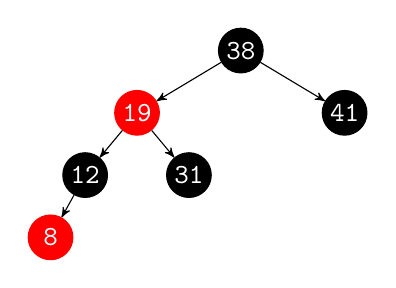
\begin{tikzpicture}[->,>=stealth',level/.style={sibling distance = 7.5em/#1,
        level distance = 2.25em}]
        \node [BlackNode] {38}
            child{ node [RedNode] {19}
                child{ node [BlackNode] {12}
                    child{ node [RedNode] {8}}
                    child{ node [] {} edge from parent [draw = none]}
                }
                child{ node [BlackNode] {31}}
            }
            child{ node [BlackNode] {41}}
    ;
    \end{tikzpicture}
    \caption{插入关键字之后的红黑树}
    \end{figure}
    \subsection*{(a)}
    依次删除关键字后得到的红黑树分别如下图
    \begin{figure}[H]
    \centering
    \begin{minipage}[t]{0.33\linewidth}
        \centering
        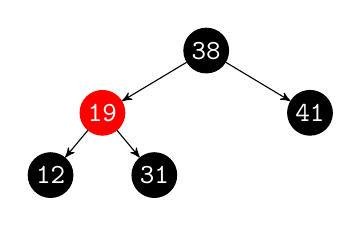
\begin{tikzpicture}[->,>=stealth',level/.style={sibling distance = 7.5em/#1,
            level distance = 2.25em}]
            \node [BlackNode] {38}
                child{ node [RedNode] {19}
                    child{ node [BlackNode] {12}}
                    child{ node [BlackNode] {31}}
                }
                child{ node [BlackNode] {41}}
            ;
        \end{tikzpicture}
        \caption{删除8之后的红黑树}
    \end{minipage}
    \hfill
    \begin{minipage}[t]{0.33\linewidth}
        \centering
        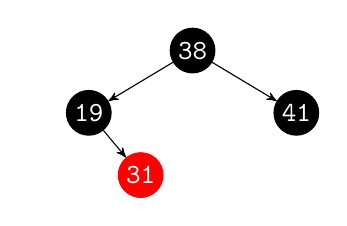
\begin{tikzpicture}[->,>=stealth',level/.style={sibling distance = 7.5em/#1,
            level distance = 2.25em}]
            \node [BlackNode] {38}
                child{ node [BlackNode] {19}
                    child{ node [] {} edge from parent [draw = none]}
                    child{ node [RedNode] {31}}
                }
                child{ node [BlackNode] {41}}
            ;
        \end{tikzpicture}
        \caption{删除12之后的红黑树}
    \end{minipage}
    \hfill
    \begin{minipage}[t]{0.33\linewidth}
        \centering
        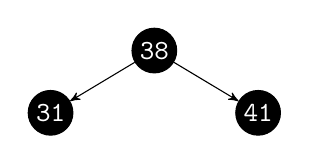
\begin{tikzpicture}[->,>=stealth',level/.style={sibling distance = 7.5em/#1,
            level distance = 2.25em}]
            \node [BlackNode] {38}
                child{ node [BlackNode] {31}}
                child{ node [BlackNode] {41}}
            ;
        \end{tikzpicture}
        \caption{删除19之后的红黑树}
    \end{minipage}
\end{figure}
\end{document}